\chapter{Hasil dan Pembahasan}
\section{Hasil Pengujian dengan satu hidden layer dengan variasi jumlah neuron}
\begin{figure}[H]
    \centering
    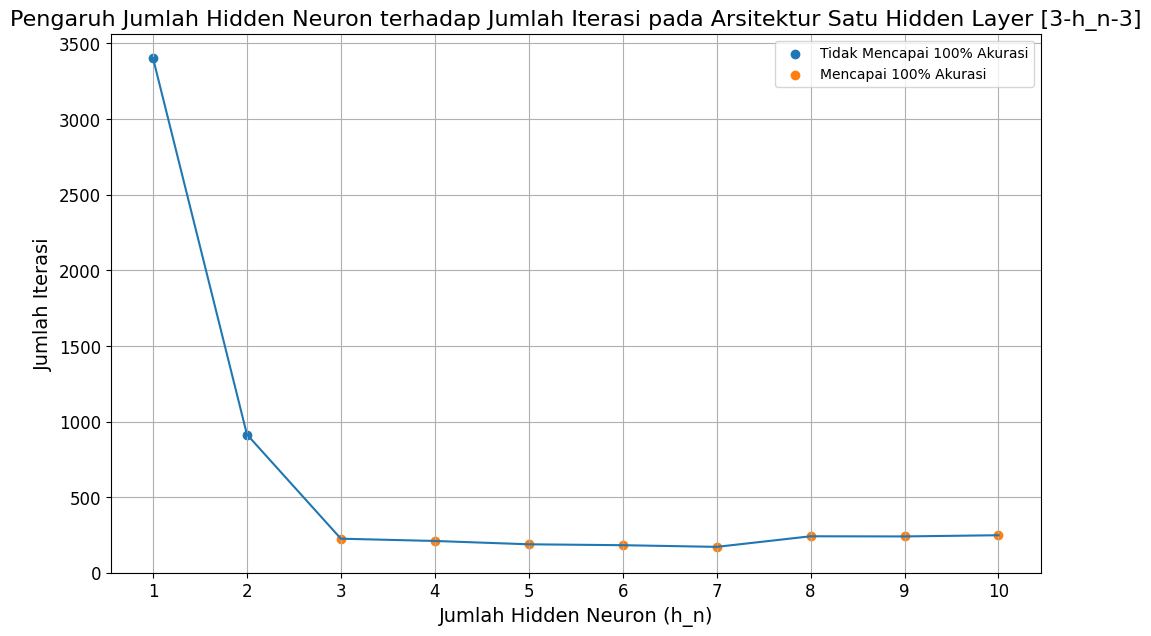
\includegraphics[width=14cm]{contents/chapter-4/1.png}
    \caption{Grafik akurasi terhadap jumlah iterasi}
    \label{fig:Plot VHN Iterasi}
\end{figure}

Pada gambar \ref{fig:Plot VHN Iterasi} terlihat pengaruh jumlah hidden neuron pada 1 hidden layer dengan arsitektur [3-h\_n-3]. Terlihat pada konfigurasi dengan 1 dan 2 hidden neuron tidak mencapai akurasi 100\%. Sedangkan pada konfigurasu 3 hingga 10 hidden neuron berhasil mencapai 100\% akurasi. Untuk melihat trend nya dapat menggunakan \textit{Polynomial Curve Fit}.

\begin{figure}[H]
    \centering
    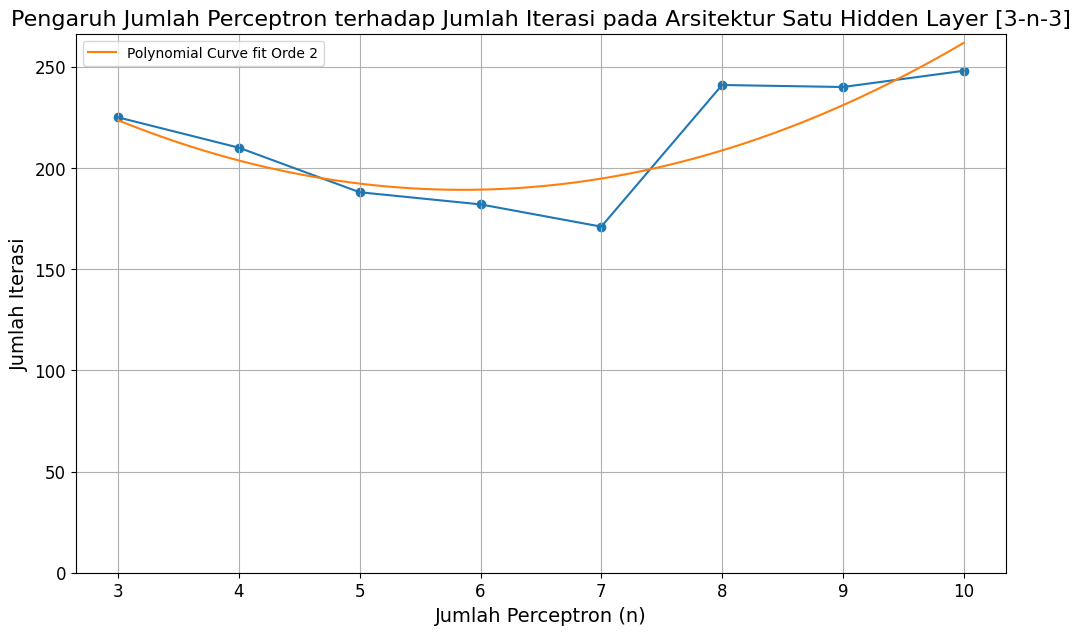
\includegraphics[width=14cm]{contents/chapter-4/2.png}
    \caption{Grafik akurasi terhadap jumlah iterasi}
    \label{fig:Plot VHN Iterasi 2}
\end{figure}

Pada gambar \ref{fig:Plot VHN Iterasi 2} akan difokuskan pada jaringan yang berhasil mencapai 100\% akurasi. Terlihat dengan menggunakan \textit{Polynomial Curve Fit} orde 2 bahwa iterasi turun seiring degan penambahan jumlah hidden neuron hingga titik tertentu, kemudian meningkat kembali.

\begin{figure}[H]
    \centering
    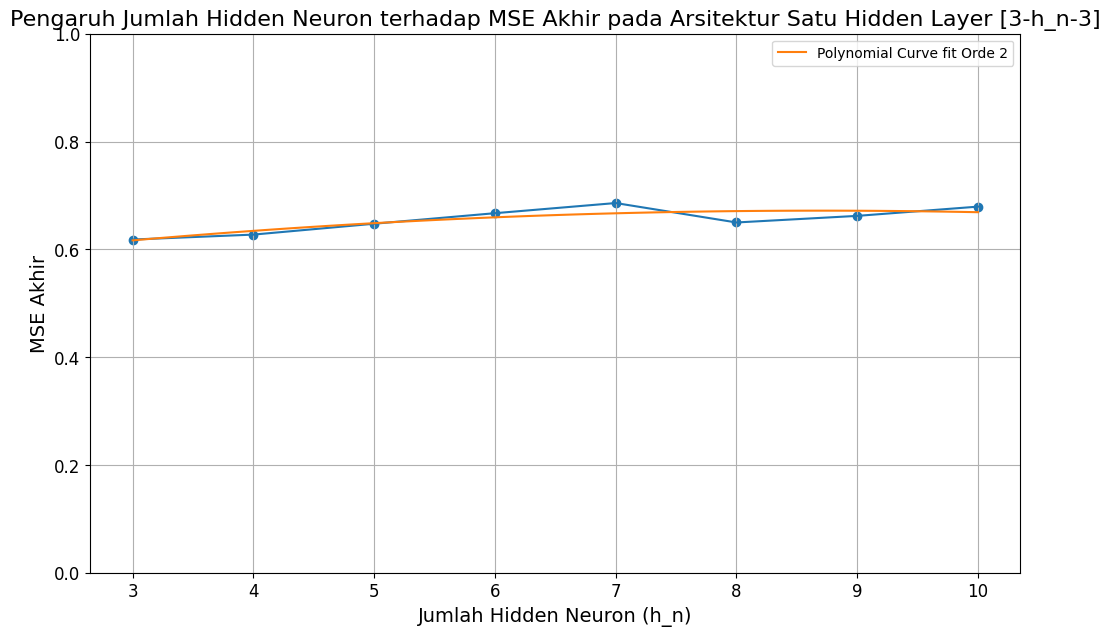
\includegraphics[width=14cm]{contents/chapter-4/3.png}
    \caption{Grafik akurasi terhadap jumlah iterasi}
    \label{fig:Plot VHN MSE}
\end{figure}

Pada gambar \ref{fig:Plot VHN MSE} terlihat bahwa nilai MSE akhir meningkat seiring dengan penurunan jumlah iterasi yang diperlukan untuk mencapai 100\% akurasi. Hal ini akan lebih terlihat jika kedua plot dibuat dalam satu figur seperti pada Gambar \ref{fig:Plot VHN MSE Akurasi}.

\begin{figure}[H]
    \centering
    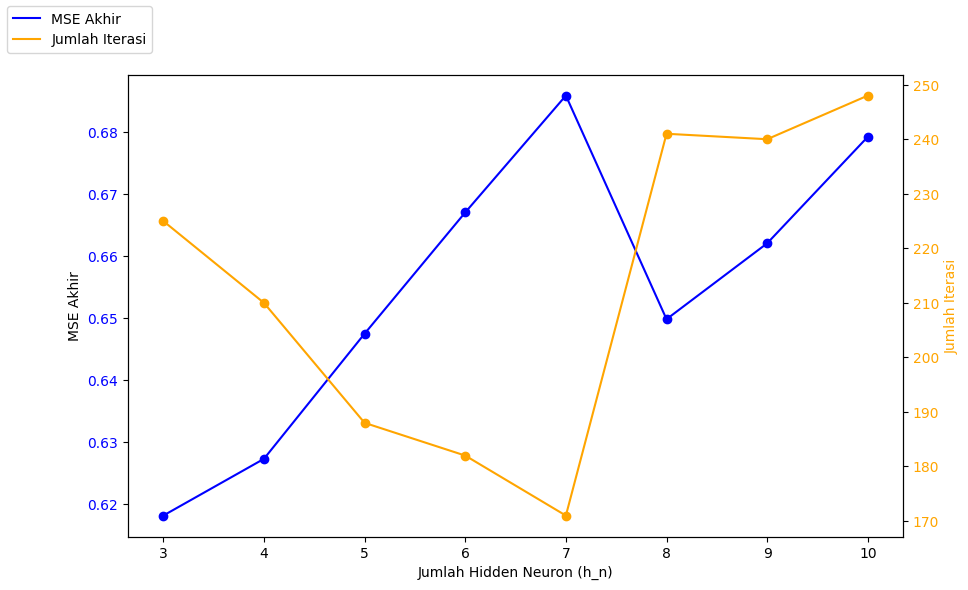
\includegraphics[width=14cm]{contents/chapter-4/4.png}
    \caption{Grafik akurasi terhadap jumlah iterasi}
    \label{fig:Plot VHN MSE Akurasi}
\end{figure}

\section{Hasil Pengujian  dengan variasi jumlah hidden layer dengan jumlah neuron yang
sama}

Pelatihan dilakukan dengan jumlah hidden layer yang bervariasi mulai dari 1 hingga 4 hidden layer dan 3 hingga 6 Hidden Neuron. Nilai awal bobot dibuat serupa untuk semua variasi yaitu sesuai dengan Persamaan \ref{eq:bobot awal}. Nilai Threshold dibuat 0.1 dan nilai \textit{learning rate} dibuat 0.1. Detail pelatihan lebih lanjut dijelaskan pada Halaman \pageref{fig:Flowchart Class}. Data hasil yang diambil berupa grafik jumlah Hidden Neuron dengan jumlah iterasinya.

\begin{figure}[H]
    \centering
    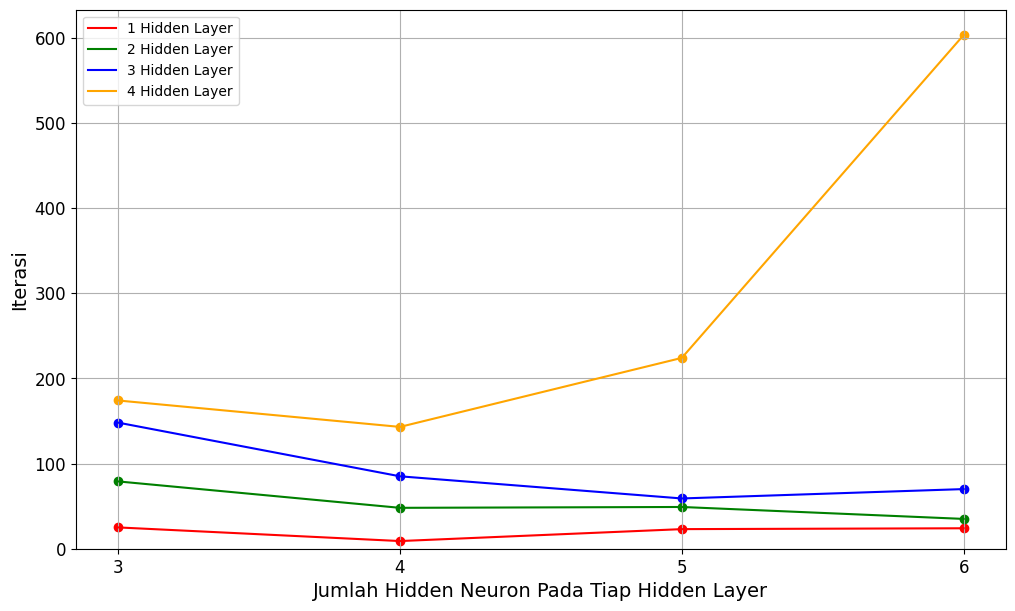
\includegraphics[width=14cm]{contents/chapter-4/5.png}
    \caption{Grafik akurasi terhadap jumlah iterasi}
    \label{fig:Grafik Akurasi}
\end{figure}

Pada Gambar \ref{fig:Grafik Akurasi} terlihat bahwa semua konfigurasi dari 1 hidden layer hingga 4 hidden layer mencapai 100\% akurasi. Terlihat bahwa semakin banyak \textit{hidden layer} semakin banyak pula iterasi yang diperlukan. Dan dengan konfigurasi 4 \textit{Hidden Layer} dengan 6 \textit{Hidden Neuron} di setiap \textit{Hidden layer}nya memiliki jumlah iterasi terbanyak. Pada konfigurasi tersebut akan memiliki 144 bobot. 

\section{Hasil Pengujian dengan variasi jumlah hidden layer dengan jumlah bobot yang
sama}

Pengujian menggunakan bobot yang sama dengan variasi jumlah Hidden Layer yang berbeda. Pemilihan bobot yang benar diperlukan karena tidak semua jumlah bobot dapat dibuat pada beberapa jumlah \textit{Hidden layer} tertentu.

\begin{figure}[H]
    \centering
    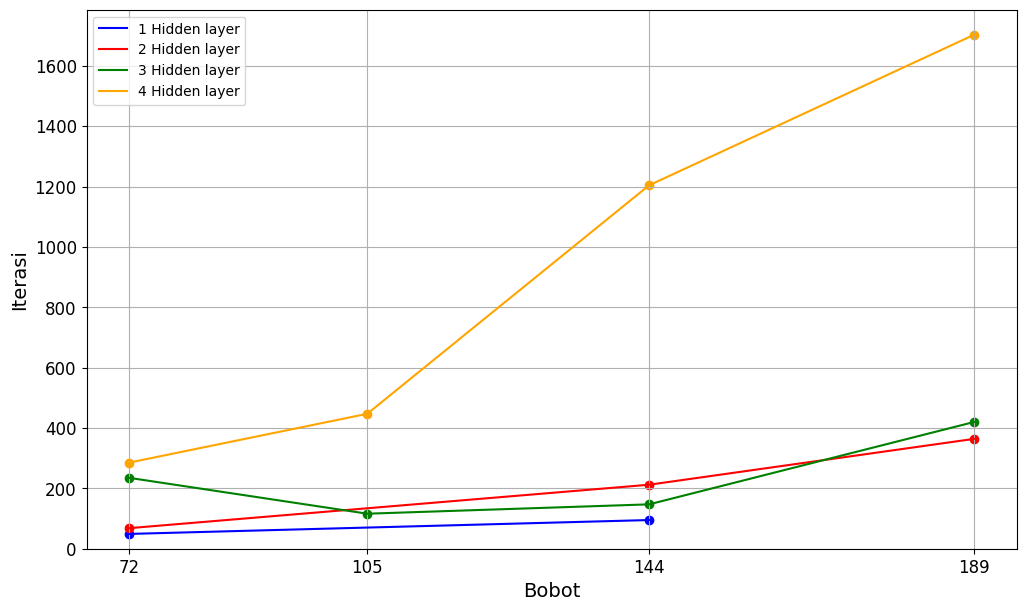
\includegraphics[width=14cm]{contents/chapter-4/6.png}
    \caption{Grafik akurasi terhadap jumlah iterasi}
    \label{fig:Grafik Akurasi 1}
\end{figure}

Sebagai contoh adalah pada Gambar \ref{fig:Grafik Akurasi 1}, terlihat bahwa bobot 105 tidak memiliki konfigurasi pada 1 dan 2 Hidden layer. Pada Jumlah bobot 189 juga tidak ditemukan konfigurasi untuk 1 Hidden layer. Berdasarkan gambar tersebut 4 hidden layer selalu memiliki jumlah iterasi terbanyak dibanding dengan konfigurasi \textit{Hidden Layer} lebih sedikit. Sedangkan dengan  konfigurasi 3 \textit{hidden layer} memiliki jumlah iterasi yang lebih tinggi dari 1 atau 2 hidden layer kecuali pada jumlah bobot 144 dan selalu lebih rendah dari 4 jumlah hidden layer. 
